\documentclass[submit]{../harvardml}
\usepackage{../common}

\course{CS1810-S26}
\assignment{Homework \#1}
\duedate{February 13, 2026 at 11:59 PM}

\usepackage[OT1]{fontenc}
\usepackage[colorlinks,citecolor=blue,urlcolor=blue]{hyperref}
\usepackage{graphicx}
\usepackage{caption}
\usepackage{enumitem}
\usepackage{soul}
\usepackage{amsmath}
\usepackage{amssymb}
\usepackage{color}
\usepackage{todonotes}
\usepackage{listings}
\usepackage{framed}
\usepackage{float}
\usepackage{ifthen}
\usepackage{bm}


\usepackage[mmddyyyy,hhmmss]{datetime}



\definecolor{verbgray}{gray}{0.9}

\lstnewenvironment{csv}{
  \lstset{backgroundcolor=\color{verbgray},
  frame=single,
  framerule=0pt,
  basicstyle=\ttfamily,
  columns=fullflexible}}{}

 \DeclareMathOperator*{\limover}{\overline{lim}}

%%%%%%%%%%%%%%%%%%%%%%%%%%%%%%%%%%%%%%%%%%%
%% Solution environment
\usepackage{xcolor}
\newenvironment{solution}{
    \vspace{2mm}
    \color{blue}\noindent\textbf{Solution}:
}{}
%%%%%%%%%%%%%%%%%%%%%%%%%%%%%%%%%%%%%%%%%%%

\begin{document}
\begin{center}
  {\Large Regression}
\end{center}

\subsection*{Introduction}

This homework is on different three different forms of regression:
nearest neighbors regression, kernelized regression, and linear
regression.  We will discuss implementation and examine their
tradeoffs by implementing them on the same dataset, which consists of
temperature over the past 800,000 years taken from ice core samples.

The folder \verb|data| contains the data you will use for this
problem. There are two files:
\begin{itemize}
  \item \verb|earth_temperature_sampled_train.csv|
  \item \verb|earth_temperature_sampled_test.csv|
\end{itemize}

Each has two columns.  The first column is the age of the ice core
sample.  The second column is the approximate difference in a year's temperature (K)
from the average temperature of the 1,000 years preceding it. The temperatures were retrieved from ice cores in
Antarctica (Jouzel et al. 2007)\footnote{Retrieved from
  \url{https://www.ncei.noaa.gov/pub/data/paleo/icecore/antarctica/epica_domec/edc3deuttemp2007.txt}

  Jouzel, J., Masson-Delmotte, V., Cattani, O., Dreyfus, G., Falourd,
  S., Hoffmann, G., … Wolff, E. W. (2007). Orbital and Millennial
  Antarctic Climate Variability over the Past 800,000 Years.
  \emph{Science, 317}(5839), 793–796. doi:10.1126/science.1141038}.

The following is a snippet of the data file:

\begin{csv}
  # Age, Temperature
  399946,0.51
  409980,1.57
\end{csv}

\noindent And this is a visualization of the full dataset:
\begin{center}
  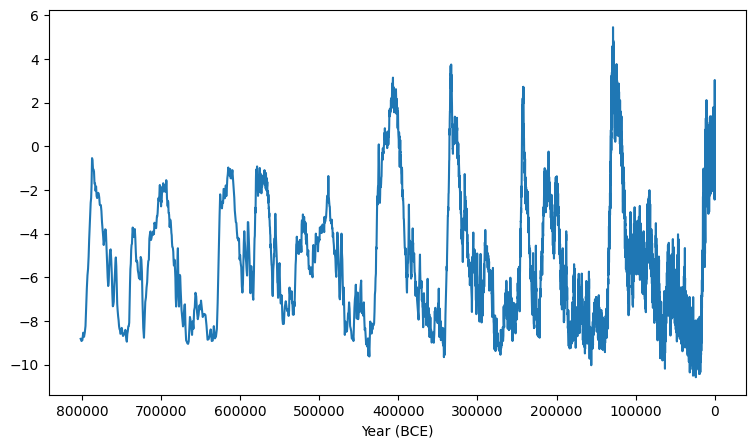
\includegraphics[width=.8\textwidth]{img_input/sample_graph}
\end{center}
\noindent


\textbf{Due to the large magnitude of the years, we will work in terms
  of thousands of years BCE in these problems.} This is taken care of
for you in the provided notebook.






\subsection*{Resources and Submission Instructions}

% The course textbook is not fully updated to the spring 2026 rendition of CS 1810, but if you want to take a look, it may still be helpful to see Sections 2.1-2.7 of the \href{https://github.com/harvard-ml-courses/cs181-textbook/blob/master/Textbook.pdf}{cs181-textbook notes}.

% We also encourage you to first read the
% \href{http://users.isr.ist.utl.pt/~wurmd/Livros/school/Bishop\%20-\%20Pattern\%20Recognition\%20And\%20Machine\%20Learning\%20-\%20Springer\%20\%202006.pdf}{Bishop textbook}, particularly: Section 2.3 (Properties of Gaussian Distributions), Section 3.1 (Linear Basis Regression), and Section 3.3 (Bayesian Linear Regression). (Note that our notation is slightly different but the underlying mathematics remains the same!).

Please type your solutions after the corresponding problems using this \LaTeX\ template, and start each main problem on a new page.

Please submit the writeup PDF to the Gradescope assignment `HW1'. Remember to assign pages for each question.  \textbf{You must include any plots in your writeup PDF. }. Please submit your \LaTeX file and code files to the Gradescope assignment `HW1 - Supplemental.' The supplemental files will only be checked in special cases, e.g. honor code issues, etc. Your files should be named in the same way as we provide them in the repository, e.g. \texttt{hw1.pdf}, etc.

If you find that you are having trouble with the first couple problems, it may be helpful to refer to Section 0 notes and review some linear algebra and matrix calculus.

\newpage

%%%%%%%%%%%%%%%%%%%%%%%%%%%%%%%%%%%%%%%%%%%%%
% Problem 1
%%%%%%%%%%%%%%%%%%%%%%%%%%%%%%%%%%%%%%%%%%%%%
\begin{problem}[kNN and Kernels, 35pts]

You will now implement two non-parametric regressions to model temperatures over time.
% For this problem, you will use the \textbf{same dataset as in Problem 1}.

\vspace{0.5cm}
\noindent\emph{Make sure to include all required plots in your PDF. Passing all test cases does not guarantee that your solution is correct, and we encourage you to write your own. }

\begin{enumerate}
\item
 Recall that kNN uses a predictor of the form
\[
  f(x^*) = \frac{1}{k} \sum_n y_n \mathbb{I}(x_n \texttt{ is one of k-closest to } x^*),
\]
where $\mathbb{I}$ is an indicator variable.
\begin{enumerate}

  \item The kNN implementation \textbf{has been provided for you} in the notebook. Run the cells to plot the results for $k=\{1, 3, N-1\}$, where $N$ is the size of the dataset. Describe how the fits change with $k$. Please include your plot in your solution PDF.

  \item Now, we will evaluate the quality of each model \emph{quantitatively} by computing the error on the provided test set. Write Python code to compute the test MSE for each value of $k$.  Report the values here. Which solution has the lowest MSE?

\end{enumerate}

\item \textit{Kernel-based regression} techniques are another form of non-parametric regression. Consider a kernel-based
regressor of the form
\begin{equation*}
  f_\tau(x^*) = \cfrac{\sum_{n} K_\tau(x_n,x^*) y_n}{\sum_n K_\tau(x_n, x^*)}
\end{equation*}
where $\mathcal{D}_\texttt{train} = \{(x_n,y_n)\}_{n = 1} ^N$ are the
training data points, and $x^*$ is the point for which you want to
make the prediction.  The kernel $K_\tau(x,x')$ is a function that
defines the similarity between two inputs $x$ and $x'$. A popular
choice of kernel is a function that decays as the distance between the
two points increases, such as
\begin{equation*}
  K_\tau(x,x') = \exp\left(-\frac{(x-x')^2}{\tau}\right)
\end{equation*}

where $\tau$ represents the square of the lengthscale (a scalar value that
dictates how quickly the kernel decays).


\begin{enumerate}

  \item First, implement the \texttt{kernel\_regressor} function in the notebook, and plot your model for years in the range $800,000$ BC to $400,000$ BC at $1000$ year intervals for the following three values of $\tau$: $1, 50, 2500$. Since we're working in terms of thousands of years, this means you should plot $(x, f_\tau(x))$ for $x = 400, 401, \dots, 800$. \textbf{In no more than 10 lines}, describe how the fits change with $\tau$. Please include your plot in your solution PDF.

  \item Denote the test set as $\mathcal{D}_\texttt{test} = \{(x'_m, y'_m)\}_{m = 1} ^M$.  Write down the expression for the MSE of $f_\tau$ over the test set as a function of the training set and test set. Your answer may include $\{(x'_m, y'_m)\}_{m = 1} ^M$, $\{(x_n, y_n)\}_{n = 1} ^N$, and $K_\tau$, but not $f_\tau$.

    \item Compute the MSE on the provided test set for the three values of $\tau$.  Report the values here. Which model yields the lowest MSE? Conceptually, why is this the case? Why would choosing $\tau$ based on $\mathcal{D}_\texttt{train}$ rather than $\mathcal{D}_\texttt{test}$ be a bad idea?

  \item Describe the time and space complexity of both kernelized regression and kNN with respect to the size of the training set $N$.  How, if at all, does the size of the model---everything that needs to be stored to make predictions---change with the size of the training set $N$?  How, if at all, do the number of computations required to make a prediction for some input $x^*$ change with the size of the training set $N$?.


  \item  What is the exact form of $\lim_{\tau \to 0 }f_\tau(x^*)$?
  \end{enumerate}
\end{enumerate}
\end{problem}

\newpage

\begin{solution}

\begin{enumerate}

%%%%%%%%%%%%%%%%%%%%%%%%%%%%%%%%%%%%%%%%%%%%%%%%%%%%%%%%%%%%%%%%%%%%%%%%%%%%%
\item % 1. kNN
\begin{enumerate}

%%%%%%%%%%%%%%%%%%%%%%%%%%%%%%%%%%%%%%%%%%%%%%%%%%%%%%%% 1(a)
\item
\begin{center}
  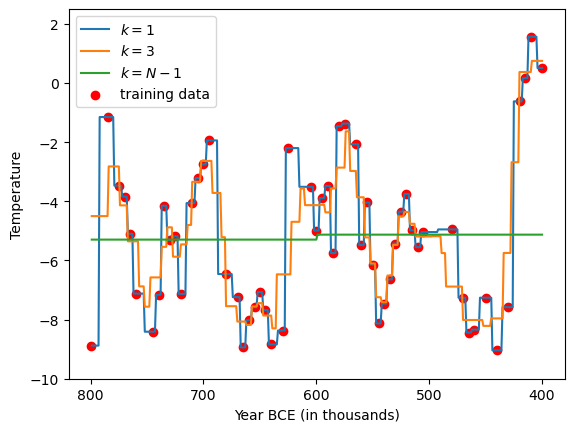
\includegraphics[width=.75\textwidth]{img_output/p1.1a.png}
\end{center}

For every $k$ the fit is a piecewise-constant step function, since the set of
$k$ nearest training points only changes as $x^*$ crosses a boundary between
neighbourhoods.

\begin{itemize}
  \item $k=1$: the prediction is the label of the single nearest training
    point, so the curve passes exactly through every training point and its
    training error is $0$. It reproduces every wiggle in the data, including
    noise --- low bias, high variance.
  \item $k=3$: each prediction is an average of three labels, so the steps are
    wider and the peaks and troughs are pulled toward one another. The fit no
    longer interpolates the data but still tracks the glacial cycles. This is a
    moderate amount of smoothing.
  \item $k=N-1$: essentially every training point is averaged for every
    $x^*$, so the fit is a nearly flat line at the global mean temperature
    ($\approx -5.1$). All structure in the data has been smoothed away --- high
    bias, near-zero variance.
\end{itemize}

So $k$ is the smoothing / complexity knob: increasing $k$ moves the model along
the bias--variance tradeoff from interpolation toward a constant predictor.

%%%%%%%%%%%%%%%%%%%%%%%%%%%%%%%%%%%%%%%%%%%%%%%%%%%%%%%%% 1(b)
\item
Test MSEs:

\begin{center}
\begin{tabular}{cc}
  \hline
  $k$ & Test MSE \\
  \hline
  $1$         & $1.7406$ \\
  $3$         & $3.8908$ \\
  $N-1 = 56$  & $9.5286$ \\
  \hline
\end{tabular}
\end{center}

$k=1$ has the lowest test MSE. The training points are spaced roughly $5$
thousand years apart and the underlying temperature signal varies on a
comparable scale, so a test point's nearest training neighbour is genuinely
informative; averaging over more neighbours here blurs across real structure
faster than it cancels noise. $k=N-1$ is close to predicting the global mean,
and its MSE ($9.53$) is therefore close to the variance of the test labels.

\end{enumerate}

%%%%%%%%%%%%%%%%%%%%%%%%%%%%%%%%%%%%%%%%%%%%%%%%%%%%%%%%%%%%%%%%%%%%%%%%%%%%%
\item % 2. Kernel regression
\begin{enumerate}

%%%%%%%%%%%%%%%%%%%%%%%%%%%%%%%%%%%%%%%%%%%%%%%%%%%%%%%%% 2(a)
\item
\begin{center}
  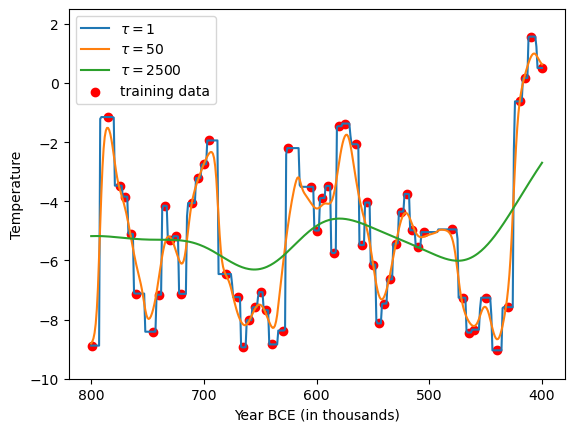
\includegraphics[width=.75\textwidth]{img_output/p1.2a.png}
\end{center}

$\tau$ is the squared lengthscale, so the kernel has effective width
$\sqrt{\tau}$ and controls how many training points meaningfully contribute to
a prediction.

\begin{itemize}
  \item $\tau = 1$ (lengthscale $1$ kyr): far narrower than the $\approx 5$ kyr
    spacing of the data. For any $x^*$ one training point dominates the
    weighted average, so the fit is a step function that interpolates the
    training data (training MSE $\approx 10^{-15}$) --- effectively 1-NN.
  \item $\tau = 50$ (lengthscale $\approx 7$ kyr): a handful of nearby points
    are averaged. The fit is smooth, passes near but not through the data, and
    still follows the glacial cycles.
  \item $\tau = 2500$ (lengthscale $50$ kyr): the weights are nearly uniform
    over the whole $400$ kyr range, so the fit is an almost flat curve near the
    global mean and all cyclical structure is lost.
\end{itemize}

Increasing $\tau$ therefore increases smoothing, moving the fit from
interpolation (high variance) to a near-constant predictor (high bias).

%%%%%%%%%%%%%%%%%%%%%%%%%%%%%%%%%%%%%%%%%%%%%%%%%%%%%%%%% 2(b)
\item
Substituting the definition of $f_\tau$ into the mean squared error over
$\mathcal{D}_\texttt{test} = \{(x'_m, y'_m)\}_{m=1}^{M}$:
\[
  \text{MSE}(\tau)
  = \frac{1}{M}\sum_{m=1}^{M}
    \left(
      y'_m - \frac{\sum_{n=1}^{N} K_\tau(x_n, x'_m)\, y_n}
                  {\sum_{n=1}^{N} K_\tau(x_n, x'_m)}
    \right)^{\!2}.
\]

%%%%%%%%%%%%%%%%%%%%%%%%%%%%%%%%%%%%%%%%%%%%%%%%%%%%%%%%% 2(c)
\item
Test MSEs:

\begin{center}
\begin{tabular}{cc}
  \hline
  $\tau$ & Test MSE \\
  \hline
  $1$     & $1.9473$ \\
  $50$    & $1.8583$ \\
  $2500$  & $8.3339$ \\
  \hline
\end{tabular}
\end{center}

$\tau = 50$ yields the lowest test MSE. Conceptually, $\sqrt{50} \approx 7$
thousand years is the right order of magnitude for this data: it is wide enough
to average over a few neighbouring samples --- cancelling measurement noise ---
but narrow enough that the averaging does not cross the $\sim 100$ kyr glacial
cycles. $\tau = 1$ overfits: it reproduces each training label, noise included,
so it inherits that noise at test time. $\tau = 2500$ underfits: it averages
across the entire record and returns something close to the global mean.

Choosing $\tau$ by minimising the error on $\mathcal{D}_\texttt{train}$ would be
a bad idea because training error is monotonically decreasing in the direction
of smaller $\tau$: as $\tau \to 0$ the predictor interpolates every training
point and the training MSE $\to 0$ (we measured $\approx 10^{-15}$ already at
$\tau = 1$). The training set therefore contains no signal about
generalisation, and the procedure would always select the most overfit model.
$\tau$ must be selected on data the model has not fit. (Strictly, selecting it
on $\mathcal{D}_\texttt{test}$ is also not ideal: once the test set is used to
choose a hyperparameter, the resulting test MSE is an optimistically biased
estimate of generalisation error. The correct practice is a held-out validation
set or cross-validation on the training data, reserving the test set for a
single final evaluation.)

%%%%%%%%%%%%%%%%%%%%%%%%%%%%%%%%%%%%%%%%%%%%%%%%%%%%%%%%% 2(d)
\item
Both are \emph{non-parametric}: there is no fitting step, and the ``model'' is
the training set itself.

\textbf{Space (model size).} Both must store all $N$ pairs $(x_n, y_n)$, so the
model size is $\Theta(N)$ --- it grows linearly and without bound in the size of
the training set. Nothing is compressed or summarised at training time.

\textbf{Time (one prediction at $x^*$).}
\begin{itemize}
  \item Kernelized regression: evaluate $K_\tau(x_n, x^*)$ for all $n$ and form
    two sums, $\Theta(N)$ operations.
  \item kNN: compute all $N$ distances, $\Theta(N)$, then select the $k$
    smallest. With a linear-time selection algorithm this is $\Theta(N)$
    overall; a naive full sort gives $\Theta(N \log N)$. The provided
    implementation sorts, so it is $\Theta(N \log N)$.
\end{itemize}

So for both methods the cost of a single prediction grows linearly (up to a log
factor for sorted kNN) with $N$. This is the characteristic tradeoff of
non-parametric methods: zero training cost, but memory and prediction cost that
scale with the data --- in contrast to a parametric model, which pays a
one-time fitting cost and then predicts in time and space independent of $N$.

%%%%%%%%%%%%%%%%%%%%%%%%%%%%%%%%%%%%%%%%%%%%%%%%%%%%%%%%% 2(e)
\item
Let $d_n = (x_n - x^*)^2$ and $d_{\min} = \min_n d_n$, and let
$S = \{ n : d_n = d_{\min}\}$ be the set of nearest training points. Multiplying
numerator and denominator by $e^{\,d_{\min}/\tau}$,
\[
  f_\tau(x^*)
  = \frac{\sum_n e^{-(d_n - d_{\min})/\tau} y_n}
         {\sum_n e^{-(d_n - d_{\min})/\tau}}.
\]
For $n \in S$ the exponent is $0$, so the term is $1$. For $n \notin S$ we have
$d_n - d_{\min} > 0$, so $e^{-(d_n - d_{\min})/\tau} \to 0$ as $\tau \to 0^+$.
Hence
\[
  \boxed{\;
  \lim_{\tau \to 0^+} f_\tau(x^*)
  = \frac{1}{|S|}\sum_{n \in S} y_n,
  \qquad S = \argmin_n |x_n - x^*| \;}
\]
i.e.\ the average of the labels of the training points nearest to $x^*$. When
the nearest neighbour is unique --- which holds for all but a measure-zero set
of $x^*$ --- this is simply $y_{n^*}$ with $n^* = \argmin_n |x_n - x^*|$, so
the limiting predictor is exactly 1-nearest-neighbour regression. (Verified
numerically: using a log-sum-exp-stable implementation, the kernel predictions
on the test set agree with 1-NN to machine precision for all $\tau \le 10^{-2}$.)

\end{enumerate}
\end{enumerate}

\end{solution}

\newpage


%%%%%%%%%%%%%%%%%%%%%%%%%%%%%%%%%%%%%%%%%%%%%
% Problem 2
%%%%%%%%%%%%%%%%%%%%%%%%%%%%%%%%%%%%%%%%%%%%%
\begin{problem}[Geometric Least Squares, 20pts]
    Linear regression can be understood using geometric intuition in $\mathbb{R}^n$. The design matrix $\mathbf X \in \mathbb{R}^{N\times D}$, with $N > D$, spans a subspace $C(\mathbf X)$, the column space of $\mathbf X$ (referred to in lecture as column span) which is a subspace of $\mathbb{R}^N$. If you wish to review the concept of a column space, consider visiting Section 0 notes. \\

    \noindent Fitting by linear regression, sometimes called \textit{ordinary least-squares} (OLS), is just projecting the observation vector $\mathbf y \in \mathbb{R}^N$ orthogonally onto that subspace. Lecture 2 slides provide a good graphic to visualize this, see the slide titled ``Geometric Interpretation.'' From lecture, we also learned that $\hat {\mathbf y}$ lives in $C(\mathbf X)$ and the residual $\mathbf r = {\mathbf y} - \hat {\mathbf y}$ lives in the orthogonal complement.

    \begin{enumerate}
    \item Let $\mathbf X \in \mathbb{R}^{N\times D}$ have full column rank $d$ and $\mathbf y \in \mathbb{R}^N$. Let the OLS estimator be $\mathbf w^*=(\mathbf X^\top \mathbf X)^{-1} X^\top \mathbf y$ and the fitted vector $\mathbf{\hat{y}} = \mathbf X \mathbf w^*$. Prove that $\hat {\mathbf y}$ is the \textit{orthogonal projection} of $y$ onto $C(\mathbf X)$. In other words, show that $\hat {\mathbf y} \in C(\mathbf X)$ and $\mathbf y - \hat {\mathbf y}$ is orthogonal to $C(\mathbf X)$. \textit{Hint: To show orthogonality, look at the gradient of $\mathcal L$, the loss, with respect to $\mathbf w$}.

    \item Prove that among all vectors in $C(\mathbf X)$, the fitted vector $\hat {\mathbf y}$ minimizes the Euclidean distance to $\mathbf y$. In other words, that for every vector $\mathbf v \in C(\mathbf X)$:
    \begin{equation*}
        \|\mathbf y - \hat {\mathbf y}\|_2^2 \leq \|\mathbf y - \mathbf v\|_2^2
    \end{equation*}
    Looking back at lecture, this is the formal proof of the phenomenon discussed in the image. \textit{Hint: For two vectors, $\mathbf v,\mathbf w$, if $\mathbf v$ is orthogonal to $\mathbf w$, denoted as $\mathbf v \perp \mathbf w$, then $\|\mathbf v-\mathbf w\|^2_2 = \|\mathbf v\|_2^2+\|\mathbf w\|^2_2$ (Pythagorean theorem).}

    \item In lecture, we defined the projection matrix, $\mathbf P = \mathbf X(\mathbf X^\top \mathbf X)^{-1} \mathbf X^\top$, which projects onto the subspace $C(\boldX)$. The matrix $\mathbf P$ is often called the \textit{hat matrix} because it maps $\mathbf y$ to its fitted values $\hat {\mathbf y} = \mathbf P \mathbf y$, i.e., it ``puts a hat" on $\mathbf y$. Prove the following properties of $\mathbf P$:
    \begin{itemize}
        \item Symmetry: $\mathbf P^\top = \mathbf P$
        \item Idempotence: $\mathbf P^2 = \mathbf P$
        \item Rank and Trace: $\mathrm{rank}(\mathbf P) = d$ and $\mathrm{trace}(\mathbf P) = d$.
    \end{itemize}
    % Also, provide geometric interpretation of the first two properties.
    \textit{Hint: You may use the fact that any idempotent matrix has equal rank and trace. You do not need to prove this, but it may be helpful to think about why this is true.}

    \item Suppose you fit your model as in Problem 5.1. You observe that the \textbf{residual plot} exhibits a clear parabolic (U-shaped) pattern rather than random scatter around zero (as seen in lecture). Give a geometric interpretation of this phenomenon in terms of projection onto the column space of the design matrix. Also, explain how adding a quadratic basis function affects the geometry of the regression problem and the residuals.
        \begin{figure}[H]
            \centering
            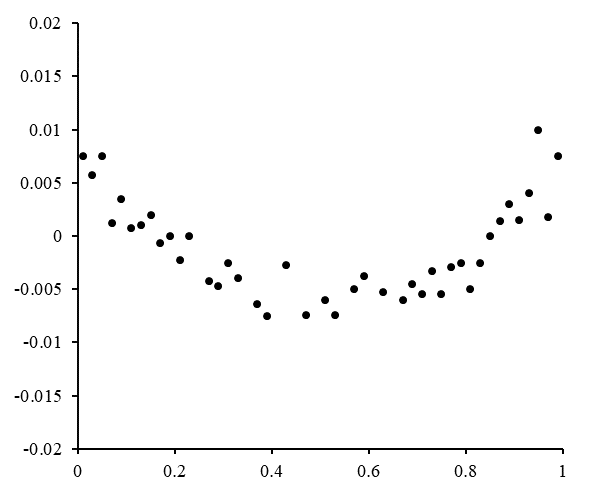
\includegraphics[scale=0.7]{img_input/residual_plot.png}
            \caption{An example residual plot with the input variable $x$ on the horizontal axis and residuals $y-\hat{y}$ on the vertical axis.}

          \end{figure}
    \end{enumerate}
\end{problem}

\newpage

\begin{solution}

%% Note on notation: the problem states $\mathbf X \in \mathbb{R}^{N \times D}$
%% has full column rank $d$; full column rank means $d = D$, and we use $d$
%% throughout to match the problem statement.

\begin{enumerate}

%%%%%%%%%%%%%%%%%%%%%%%%%%%%%%%%%%%%%%%%%%%%%%%%%%%%%%%%%%%%%%%%%%%%%%%% 2.1
\item
Since $\mathbf X$ has full column rank $d$, $\mathbf X^\top \mathbf X \in
\mathbb{R}^{d \times d}$ is invertible, so $\mathbf w^*$ is well defined.
We must show two things.

\textbf{(i) $\hat{\mathbf y} \in C(\mathbf X)$.}
By definition $\hat{\mathbf y} = \mathbf X \mathbf w^*$. Writing $\mathbf X =
[\tilde{\mathbf x}_1 \;\cdots\; \tilde{\mathbf x}_d]$ in terms of its columns,
\[
  \hat{\mathbf y} = \mathbf X \mathbf w^* = \sum_{j=1}^{d} w^*_j \tilde{\mathbf x}_j ,
\]
which is a linear combination of the columns of $\mathbf X$ and hence lies in
$C(\mathbf X)$ by definition of the column space.

\textbf{(ii) $\mathbf r := \mathbf y - \hat{\mathbf y}$ is orthogonal to
$C(\mathbf X)$.}
Following the hint, the least-squares loss is
$\mathcal L(\mathbf w) = \|\mathbf y - \mathbf X \mathbf w\|_2^2
 = (\mathbf y - \mathbf X\mathbf w)^\top(\mathbf y - \mathbf X \mathbf w)$,
whose gradient is
\[
  \nabla_{\mathbf w}\mathcal L(\mathbf w)
  = -2\,\mathbf X^\top(\mathbf y - \mathbf X \mathbf w).
\]
Setting this to $\mathbf 0$ gives the \emph{normal equations}
$\mathbf X^\top \mathbf X \mathbf w = \mathbf X^\top \mathbf y$, whose unique
solution is $\mathbf w^* = (\mathbf X^\top\mathbf X)^{-1}\mathbf X^\top \mathbf y$.
Substituting $\mathbf w^*$ directly confirms this:
\[
  \mathbf X^\top \mathbf r
  = \mathbf X^\top\!\left(\mathbf y - \mathbf X (\mathbf X^\top \mathbf X)^{-1}\mathbf X^\top \mathbf y\right)
  = \mathbf X^\top \mathbf y - \underbrace{(\mathbf X^\top \mathbf X)(\mathbf X^\top \mathbf X)^{-1}}_{=\;\mathbf I_d}\mathbf X^\top \mathbf y
  = \mathbf 0 .
\]
Now take any $\mathbf v \in C(\mathbf X)$. By definition $\mathbf v = \mathbf X
\mathbf a$ for some $\mathbf a \in \mathbb{R}^d$, so
\[
  \mathbf v^\top \mathbf r = (\mathbf X\mathbf a)^\top \mathbf r
  = \mathbf a^\top \underbrace{\mathbf X^\top \mathbf r}_{=\;\mathbf 0} = 0 .
\]
Hence $\mathbf r \perp \mathbf v$ for every $\mathbf v \in C(\mathbf X)$, i.e.\
$\mathbf r \in C(\mathbf X)^\perp$.

Together, (i) and (ii) say that $\mathbf y$ decomposes as
$\mathbf y = \hat{\mathbf y} + \mathbf r$ with $\hat{\mathbf y} \in C(\mathbf X)$
and $\mathbf r \in C(\mathbf X)^{\perp}$, which is precisely the statement that
$\hat{\mathbf y}$ is the orthogonal projection of $\mathbf y$ onto
$C(\mathbf X)$. (This decomposition is unique, since
$\mathbb{R}^N = C(\mathbf X) \oplus C(\mathbf X)^\perp$.) $\blacksquare$

%%%%%%%%%%%%%%%%%%%%%%%%%%%%%%%%%%%%%%%%%%%%%%%%%%%%%%%%%%%%%%%%%%%%%%%% 2.2
\item
Let $\mathbf v \in C(\mathbf X)$ be arbitrary. Add and subtract
$\hat{\mathbf y}$:
\[
  \mathbf y - \mathbf v = \underbrace{(\mathbf y - \hat{\mathbf y})}_{=\;\mathbf r}
   + (\hat{\mathbf y} - \mathbf v).
\]
Because $C(\mathbf X)$ is a subspace and both $\hat{\mathbf y}$ and $\mathbf v$
lie in it, the difference $\hat{\mathbf y} - \mathbf v \in C(\mathbf X)$. By
part 1, $\mathbf r \perp C(\mathbf X)$, and therefore
$\mathbf r \perp (\hat{\mathbf y} - \mathbf v)$.

Applying the Pythagorean theorem to these two orthogonal vectors,
\[
  \|\mathbf y - \mathbf v\|_2^2
  = \|\mathbf r\|_2^2 + \|\hat{\mathbf y} - \mathbf v\|_2^2
  = \|\mathbf y - \hat{\mathbf y}\|_2^2 + \underbrace{\|\hat{\mathbf y} - \mathbf v\|_2^2}_{\ \geq\ 0}
  \;\geq\; \|\mathbf y - \hat{\mathbf y}\|_2^2 .
\]
So $\|\mathbf y - \hat{\mathbf y}\|_2^2 \leq \|\mathbf y - \mathbf v\|_2^2$ for
every $\mathbf v \in C(\mathbf X)$, as required. Moreover equality holds if and
only if $\|\hat{\mathbf y} - \mathbf v\|_2^2 = 0$, i.e.\ $\mathbf v =
\hat{\mathbf y}$, so $\hat{\mathbf y}$ is the \emph{unique} closest point in
$C(\mathbf X)$ to $\mathbf y$. $\blacksquare$

%%%%%%%%%%%%%%%%%%%%%%%%%%%%%%%%%%%%%%%%%%%%%%%%%%%%%%%%%%%%%%%%%%%%%%%% 2.3
\item
Throughout, write $\mathbf A = \mathbf X^\top \mathbf X$, which is symmetric
($\mathbf A^\top = (\mathbf X^\top\mathbf X)^\top = \mathbf X^\top \mathbf X = \mathbf A$)
and invertible (full column rank). Note that the inverse of a symmetric
invertible matrix is symmetric:
$(\mathbf A^{-1})^\top = (\mathbf A^\top)^{-1} = \mathbf A^{-1}$.

\textbf{Symmetry.} Using $(\mathbf{ABC})^\top = \mathbf C^\top\mathbf B^\top \mathbf A^\top$,
\[
  \mathbf P^\top
  = \left(\mathbf X \mathbf A^{-1} \mathbf X^\top\right)^\top
  = (\mathbf X^\top)^\top (\mathbf A^{-1})^\top \mathbf X^\top
  = \mathbf X \mathbf A^{-1}\mathbf X^\top
  = \mathbf P .
\]

\textbf{Idempotence.}
\[
  \mathbf P^2
  = \mathbf X \mathbf A^{-1}\mathbf X^\top \cdot \mathbf X \mathbf A^{-1}\mathbf X^\top
  = \mathbf X \mathbf A^{-1}\underbrace{\left(\mathbf X^\top \mathbf X\right)}_{=\;\mathbf A}\mathbf A^{-1}\mathbf X^\top
  = \mathbf X \underbrace{\mathbf A^{-1}\mathbf A}_{=\;\mathbf I_d}\mathbf A^{-1}\mathbf X^\top
  = \mathbf X \mathbf A^{-1}\mathbf X^\top = \mathbf P .
\]

\textbf{Rank.} We show $C(\mathbf P) = C(\mathbf X)$.
\begin{itemize}
  \item[($\subseteq$)] For any $\mathbf v \in \mathbb{R}^N$,
    $\mathbf P \mathbf v = \mathbf X\left(\mathbf A^{-1}\mathbf X^\top \mathbf v\right)$
    is a linear combination of the columns of $\mathbf X$, so
    $\mathbf P\mathbf v \in C(\mathbf X)$.
  \item[($\supseteq$)] For any $\mathbf v \in C(\mathbf X)$, write
    $\mathbf v = \mathbf X\mathbf a$. Then
    $\mathbf P \mathbf v = \mathbf X \mathbf A^{-1}\mathbf X^\top \mathbf X \mathbf a
     = \mathbf X\mathbf A^{-1}\mathbf A\,\mathbf a = \mathbf X \mathbf a = \mathbf v$,
    so $\mathbf v \in C(\mathbf P)$. (In words: $\mathbf P$ acts as the identity
    on $C(\mathbf X)$.)
\end{itemize}
Hence $\mathrm{rank}(\mathbf P) = \dim C(\mathbf P) = \dim C(\mathbf X)
= \mathrm{rank}(\mathbf X) = d$.

\textbf{Trace.} By the cyclic property of the trace,
$\mathrm{trace}(\mathbf{BC}) = \mathrm{trace}(\mathbf{CB})$, taking
$\mathbf B = \mathbf X$ and $\mathbf C = \mathbf A^{-1}\mathbf X^\top$:
\[
  \mathrm{trace}(\mathbf P)
  = \mathrm{trace}\!\left(\mathbf X \mathbf A^{-1}\mathbf X^\top\right)
  = \mathrm{trace}\!\left(\mathbf A^{-1}\mathbf X^\top \mathbf X\right)
  = \mathrm{trace}\!\left(\mathbf A^{-1}\mathbf A\right)
  = \mathrm{trace}(\mathbf I_d) = d .
\]
This is consistent with the hint: $\mathbf P$ is idempotent, so its eigenvalues
satisfy $\lambda^2 = \lambda$, i.e.\ $\lambda \in \{0,1\}$; since $\mathbf P$ is
also symmetric it is diagonalisable, so its trace equals the number of unit
eigenvalues, which equals the dimension of its image, i.e.\ its rank. Hence
$\mathrm{rank}(\mathbf P) = \mathrm{trace}(\mathbf P) = d$. $\blacksquare$

\medskip
\noindent\emph{Geometric reading.} Idempotence says that once a vector has been
projected into $C(\mathbf X)$, projecting again does nothing --- it is already in
the subspace. Symmetry is what makes the projection \emph{orthogonal} rather
than oblique: it is equivalent to $\langle \mathbf P\mathbf u, \mathbf v\rangle =
\langle \mathbf u, \mathbf P\mathbf v\rangle$, so the projection direction is
perpendicular to $C(\mathbf X)$. And $\mathrm{trace}(\mathbf P) = d$ is the
familiar statement that an OLS fit with $d$ features uses up $d$ ``degrees of
freedom,'' leaving $N - d$ for the residual.

%%%%%%%%%%%%%%%%%%%%%%%%%%%%%%%%%%%%%%%%%%%%%%%%%%%%%%%%%%%%%%%%%%%%%%%% 2.4
\item
\textbf{Geometric interpretation of the U-shaped residual plot.}
By part 1 the residual vector $\mathbf r = \mathbf y - \hat{\mathbf y} =
(\mathbf I - \mathbf P)\mathbf y$ lies in $C(\mathbf X)^\perp$, so it is
orthogonal to \emph{every column of} $\mathbf X$ --- in particular
$\mathbf 1^\top \mathbf r = 0$ (residuals sum to zero) and
$\tilde{\mathbf x}^\top\mathbf r = 0$ (residuals are uncorrelated with $x$).
Crucially, this guarantees orthogonality only to the $d$ directions we actually
included; it says nothing about orthogonality to \emph{other} functions of $x$.

A clean parabolic pattern means exactly that: the residual has a large
component along the direction
$\mathbf x^2 := (x_1^2, x_2^2, \ldots, x_N^2)^\top$, and $\mathbf x^2 \notin
C(\mathbf X)$. Geometrically, $\mathbf y$ has a systematic component that points
\emph{out of} the column space, and orthogonal projection onto $C(\mathbf X)$
simply threw it away into the residual. The residual is therefore not random
noise but a deterministic signal that the chosen subspace was too small to
reach --- the hallmark of \textbf{underfitting / model misspecification}. The
subspace $C(\mathbf X)$ is ``tilted the wrong way'' relative to $\mathbf y$: no
choice of $\mathbf w$ can capture the curvature, because curvature is not
expressible as a linear combination of the columns we gave the model.

\textbf{Effect of adding a quadratic basis function.}
Let the new design matrix be $\mathbf X' = [\,\mathbf X \;\; \mathbf x^2\,]
\in \mathbb{R}^{N\times(d+1)}$, with projection matrix $\mathbf P'$. Since
$\mathbf x^2 \notin C(\mathbf X)$, this strictly enlarges the subspace:
\[
  C(\mathbf X) \subsetneq C(\mathbf X'), \qquad \dim C(\mathbf X') = d+1 .
\]
Three consequences follow:

\begin{itemize}
  \item \textbf{The U-shape disappears.} The new residual
    $\mathbf r' = (\mathbf I - \mathbf P')\mathbf y$ is orthogonal to all of
    $C(\mathbf X')$, which now \emph{contains} the direction $\mathbf x^2$.
    So $(\mathbf x^2)^\top \mathbf r' = 0$: the quadratic component that
    previously sat in the residual has been absorbed into the fit, and the plot
    should return to unstructured scatter about zero.
  \item \textbf{The residual can only shrink.} Because
    $C(\mathbf X) \subseteq C(\mathbf X')$, part 2 applied to the larger
    subspace gives
    $\|\mathbf y - \mathbf P'\mathbf y\|_2^2 \leq \|\mathbf y - \mathbf P\mathbf y\|_2^2$,
    since $\mathbf P\mathbf y$ is one of the candidate vectors
    $\mathbf v \in C(\mathbf X')$ over which $\mathbf P'\mathbf y$ minimises.
    Training MSE is thus non-increasing when a basis function is added.
  \item \textbf{One more degree of freedom is spent.} The residual now lives in
    a space of dimension $N - (d+1)$ instead of $N - d$, and
    $\mathrm{trace}(\mathbf P') = d+1$. This is also the caution: each added
    basis function shrinks the residual space by one dimension, and if we keep
    adding until $D = N$ then $C(\mathbf X') = \mathbb{R}^N$, $\mathbf P' =
    \mathbf I$, and $\mathbf r' = \mathbf 0$ --- a perfect training fit that
    has interpolated the noise. A structured residual plot is a signal to add
    the \emph{specific} basis direction the structure suggests, not to add
    bases indiscriminately.
\end{itemize}

\end{enumerate}

\end{solution}

\newpage

%%%%%%%%%%%%%%%%%%%%%%%%%%%%%%%%%%%%%%%%%%%%%
% Problem 3
%%%%%%%%%%%%%%%%%%%%%%%%%%%%%%%%%%%%%%%%%%%%%

\begin{problem}[Basis Regression, 30pts]
    We now implement some linear regression models for the temperature. If we just directly use the data as given to us, we would only have a one dimensional input to our model, the year.  To create a more expressive linear model, we will introduce basis functions.

    \vspace{1em}

    \noindent\emph{Make sure to include all required plots in your PDF.}

    \begin{enumerate}
        \item We will first implement the four basis regressions below. Note that we introduce an addition transform $f$ (already into the provided notebook) to address concerns about numerical instabilities.

        \begin{enumerate}
            \item $\phi_j(x)= f(x)^j$ for $j=1,\ldots, 9$. $f(x) = \frac{x}{1.81 \cdot 10^{2}}.$

            \item $\phi_j(x) = \exp\left\{-\cfrac{(f(x)-\mu_j)^2}{5}\right\}$ for $\mu_j=\frac{j + 7}{8}$ with $j=1,\ldots, 9$. $f(x) = \frac{x}{4.00 \cdot 10^{2}}.$

            \item $\phi_j(x) =  \cos(f(x) / j)$ for $j=1, \ldots, 9$. $f(x) = \frac{x}{1.81}$.

            \item $\phi_j(x) = \cos(f(x) / j)$ for $j=1, \ldots, 49$. $f(x) = \frac{x}{1.81 \cdot 10^{-1}}$. \footnote{For the trigonometric bases (c) and (d), the periodic nature of cosine requires us to transform the data such that the lengthscale is within the periods of each element of our basis.}
        \end{enumerate}

        {\footnotesize *Note: Please make sure to add a bias term for all your basis functions above in your implementation of the \verb|make_basis|.}

        Let
        $$ \mathbf{\phi}(\mathbf{X}) = \begin{bmatrix}
            \mathbf{\phi}(x_1) \\
            \mathbf{\phi}(x_2) \\
            \vdots             \\
            \mathbf{\phi}(x_N) \\
        \end{bmatrix} \in \mathbb{R}^{N\times D}. $$
        You will complete the \verb|make_basis| function which must return $\phi(\mathbf{X})$ for each part (a) - (d). You do NOT need to submit this code in your \LaTeX writeup.

        Then, create a plot of the fitted regression line for each basis against a scatter plot of the training data. Boilerplate plotting code is provided in the notebook---you will only need to finish up a part of it. \textbf{All you need to include in your writeup for this part are these four plots.}

        \item Now we have trained each of our basis regressions. For each basis regression, compute the MSE on the test set. Discuss: do any of the bases seem to overfit? Underfit? Why?

        \item Briefly describe what purpose the transforms $\phi$ serve: why are they helpful?

        \item As in Problem 1, describe the space and time complexity of linear regression.  How does what is stored to compute predictions change with the size of the training set $N$ and the number of features $D$?  How does the computation needed to compute the prediction for a new input depend on the size of the training set $N$?  How do these complexities compare to those of the kNN and kernelized regressor?

        \item Briefly compare and constrast the different regressors: kNN, kernelized regression, and linear regression (with bases). Are some regressions clearly worse than others?  Is there one best regression?  How would you use the fact that you have these multiple regression functions?
    \end{enumerate}

    \noindent \textit{Note:} You may be concerned that we are using a different set of inputs $\mathbf{X}$ for each basis (a)-(d), since it could seem as though this prevents us from being able to directly compare the MSE of the models since we are using different data as input. But this is not an issue, since each transformation is considered as being a part of our model. This contrasts with transformations that cause the variance of the target $\mathbf{y}$ to be different  (such as standardization); in these cases the MSE can no longer be directly compared.
\end{problem}

\newpage

\begin{solution}

\begin{enumerate}

%%%%%%%%%%%%%%%%%%%%%%%%%%%%%%%%%%%%%%%%%%%%%%%%%%%%%%%%%%%%%%%%%%%%%%%% 3.1
\item
The fitted OLS regression line for each of the four bases, plotted against the
training data:
\begin{center}
  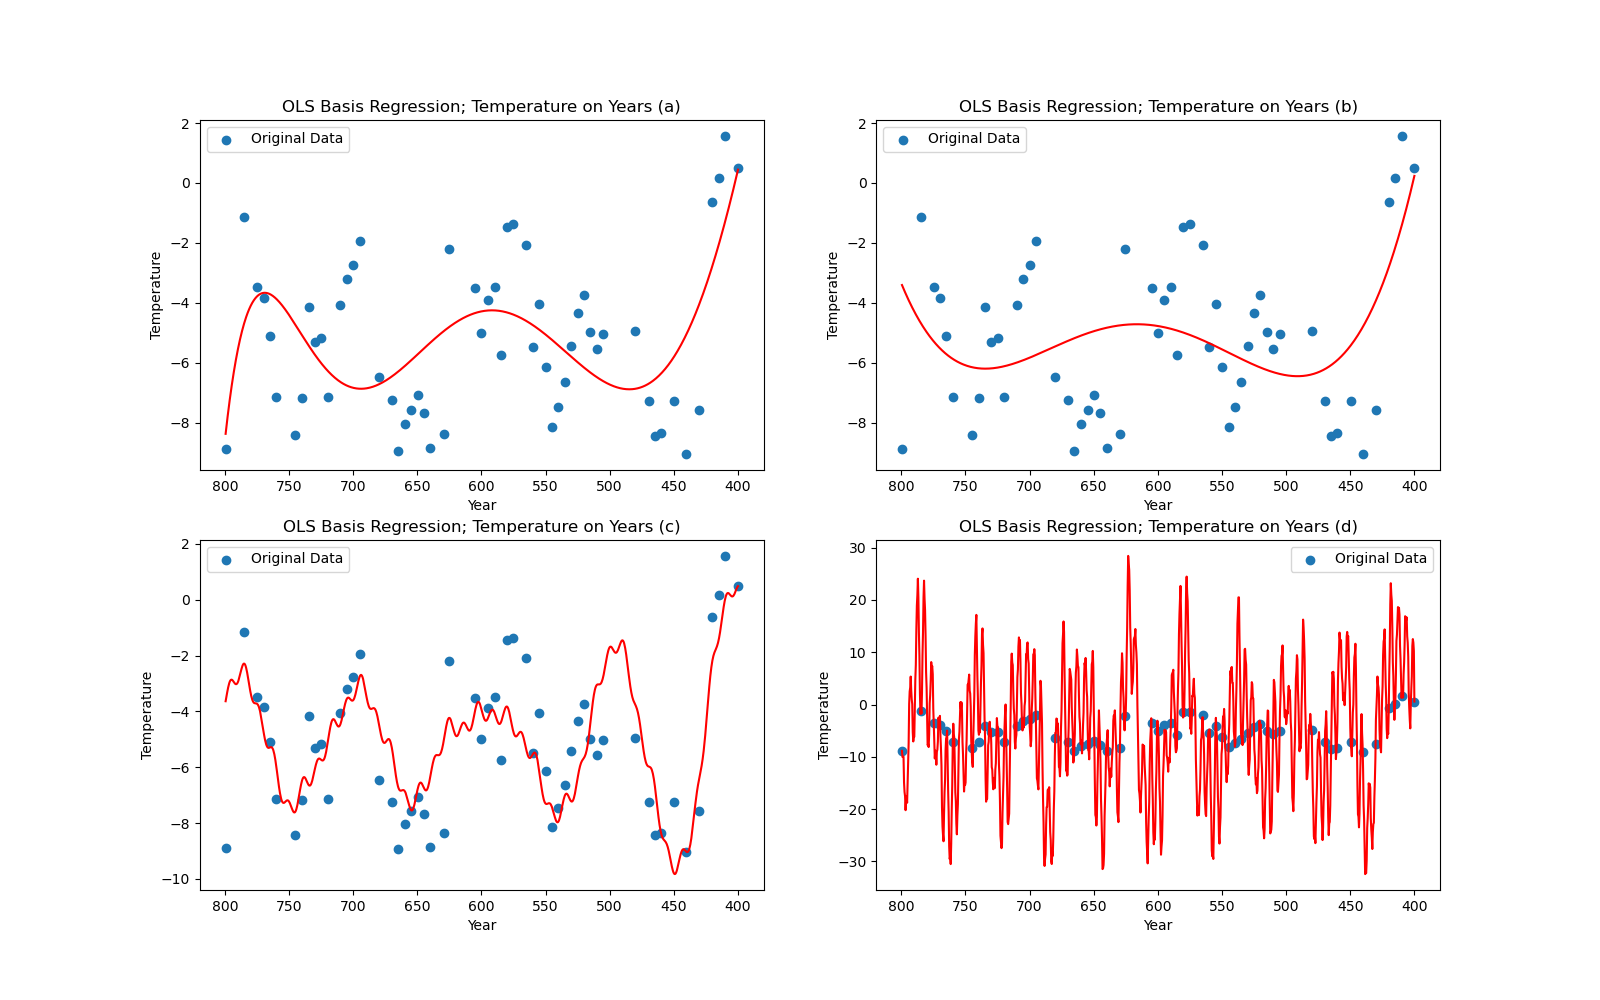
\includegraphics[width=\textwidth]{img_output/p3.1.png}
\end{center}

%%%%%%%%%%%%%%%%%%%%%%%%%%%%%%%%%%%%%%%%%%%%%%%%%%%%%%%%%%%%%%%%%%%%%%%% 3.2
\item
Training and test MSE for each basis (training MSE included since the
comparison between the two is what diagnoses over- and underfitting):
\begin{center}
\begin{tabular}{lccc}
  \hline
  Basis & $D$ (incl.\ bias) & Train MSE & Test MSE \\
  \hline
  (a) polynomial, $j=1..9$   & $10$ & $4.8248$ & $7.9558$ \\
  (b) RBF, $j=1..9$          & $10$ & $5.5300$ & $8.7081$ \\
  (c) cosine, $j=1..9$       & $10$ & $2.8791$ & $\mathbf{5.9670}$ \\
  (d) cosine, $j=1..49$      & $50$ & $\mathbf{0.6432}$ & $58.9446$ \\
  \hline
\end{tabular}
\end{center}

\noindent A useful reference point: the variance of the test labels is $9.07$,
which is the MSE a model that simply predicts the test mean would achieve.

\textbf{Basis (d) badly overfits.} It has the lowest training MSE by a wide
margin ($0.64$) and by far the worst test MSE ($58.94$) --- roughly $6.5\times$
worse than predicting a constant. With $D = 50$ parameters fit to only $N = 57$
training points, the model has nearly enough freedom to interpolate the
training set, so it fits the noise rather than the signal. The fitted weights
are enormous ($\|\mathbf w\|_2 \approx 3.9\times 10^{5}$): the high-frequency
cosines are nearly linearly dependent on this input range, so OLS cancels huge
positive and negative contributions against one another. That cancellation is
exact at the training points but falls apart everywhere else, which is the wild
oscillation visible in panel (d).

\textbf{Bases (a) and (b) underfit.} Their test MSEs ($7.96$ and $8.71$) are
both close to the $9.07$ constant-predictor baseline, so they explain very
little of the variation, and their training MSEs are also high --- high error on
\emph{both} splits is the signature of underfitting. Basis (b) is the worst of
the two: with $f(x) = x/400 \in [1, 2]$ but a bump width of
$\sqrt{5} \approx 2.24$, every radial basis function is far wider than the
entire span of the data, so the nine bumps are nearly indistinguishable from one
another. The design matrix has numerical rank $7$ rather than $10$, and only
very smooth, nearly-linear functions are reachable. Basis (a) is a degree-9
polynomial, which is more flexible but \emph{global}: each coefficient affects
the whole domain, so it cannot track several repeated glacial cycles at once,
and the design matrix is severely ill-conditioned ($\kappa \approx 7\times
10^{12}$).

\textbf{Basis (c) is the best of the four}, with the lowest test MSE ($5.97$)
and the smallest gap between train and test error relative to its scale. A
cosine basis is well matched to data that is genuinely oscillatory, and with
only $9$ frequencies it cannot chase individual points. It is also by far the
best conditioned design matrix ($\kappa \approx 2.2$), so the weights stay small
($\|\mathbf w\|_2 \approx 6.3$).

\noindent Comparing (c) and (d) isolates the effect of model complexity
cleanly: the two use the \emph{same} family of basis functions and differ only
in how many. Going from $9$ to $49$ frequencies cuts training error by a factor
of $4.5$ while multiplying test error by a factor of $10$.

%%%%%%%%%%%%%%%%%%%%%%%%%%%%%%%%%%%%%%%%%%%%%%%%%%%%%%%%%%%%%%%%%%%%%%%% 3.3
\item
The transforms serve two distinct purposes.

\textbf{Expressiveness.} Linear regression is required to be linear in the
\emph{weights} $\mathbf w$, not in the input $x$. Applying $\phi$ first means we
can fit an arbitrarily nonlinear function of $x$ while still solving the same
linear least-squares problem, so the closed form
$\mathbf w^* = (\bPhi^\top\bPhi)^{-1}\bPhi^\top\mathbf y$ still applies. In the
language of Problem 2: with the raw one-dimensional year as input, $C(\mathbf X)$
is only a $2$-dimensional subspace of $\mathbb{R}^N$ (bias and year), so
$\hat{\mathbf y}$ is confined to straight lines --- hopeless for this data. Each
basis function adds a dimension to the column space, bringing the projection of
$\mathbf y$ closer. Which \emph{direction} it adds is set by the choice of
$\phi$, so the basis encodes our prior belief about the shape of the function:
cosines for a periodic signal, bumps for localised structure, powers for smooth
global trends. Problem 3.2 shows this choice matters more than the raw count of
basis functions.

\textbf{Numerical stability.} The additional rescaling $f$ keeps the entries of
$\bPhi$ in a sane range. Without it, basis (a) would compute $x^9$ with
$x \approx 800$, i.e.\ values around $10^{26}$, which alongside the bias column
of ones produces a design matrix so ill-conditioned that
$\bPhi^\top\bPhi$ cannot be inverted reliably. For the trigonometric bases (c)
and (d), $f$ additionally places the data inside the periods of the individual
cosines, so that the basis functions are actually distinguishable from one
another over the observed range rather than all being evaluated on a tiny arc.

%%%%%%%%%%%%%%%%%%%%%%%%%%%%%%%%%%%%%%%%%%%%%%%%%%%%%%%%%%%%%%%%%%%%%%%% 3.4
\item
Linear regression is \emph{parametric}, which changes the picture entirely
relative to Problem 1.

\textbf{Space (model size).} After fitting, everything needed to predict is the
weight vector $\mathbf w \in \mathbb{R}^D$, so the model is $\Theta(D)$ --- and
crucially \textbf{independent of $N$}. The training data can be discarded once
$\mathbf w$ is computed.

\textbf{Time (training, paid once).} Forming $\bPhi$ costs $\Theta(ND)$,
forming $\bPhi^\top\bPhi$ costs $\Theta(ND^2)$, and inverting it costs
$\Theta(D^3)$, for $\Theta(ND^2 + D^3)$ overall. This is the only place $N$
enters, and it is a one-time cost.

\textbf{Time (one prediction at $x^*$).} Evaluate $\phi(x^*)$, which is
$\Theta(D)$, then take the inner product $\mathbf w^\top \phi(x^*)$, also
$\Theta(D)$. So prediction is $\Theta(D)$ and \textbf{does not depend on $N$ at
all}.

\textbf{Comparison.} kNN and kernelized regression both require $\Theta(N)$
storage and $\Theta(N)$ time per prediction (up to a $\log N$ factor for sorted
kNN), because the training set \emph{is} the model. Linear regression instead
pays $\Theta(ND^2 + D^3)$ once up front and is then $\Theta(D)$ in both space
and time forever after. Since typically $D \ll N$, this is an enormous saving at
deployment, and it is the defining practical tradeoff between parametric and
non-parametric methods: the parametric model compresses the data into $D$
numbers, while the non-parametric one refuses to summarise and keeps everything.

%%%%%%%%%%%%%%%%%%%%%%%%%%%%%%%%%%%%%%%%%%%%%%%%%%%%%%%%%%%%%%%%%%%%%%%% 3.5
\item
Collecting the best test MSE achieved by each method on this dataset:
\begin{center}
\begin{tabular}{lcc}
  \hline
  Method & Best setting & Test MSE \\
  \hline
  kNN                 & $k = 1$       & $1.7406$ \\
  Kernelized regression & $\tau = 50$ & $1.8583$ \\
  Basis regression    & basis (c)     & $5.9670$ \\
  \hline
\end{tabular}
\end{center}

\textbf{Is one method clearly worse?} Not as a \emph{family}. Basis (d) is
clearly the worst single model here ($58.94$, far worse than predicting a
constant), but that indicts a specific bad choice of complexity, not linear
regression as such --- basis (c) from the same family does perfectly
respectably. The honest comparison is between well-chosen members of each
family, and there the two non-parametric methods win clearly on this data.

\textbf{Why the non-parametric methods win here.} The training years are
sampled densely and fairly evenly across the whole $400$--$800$ kyr range, so
every test point has a genuinely nearby training point, which is exactly the
regime where local averaging excels. Meanwhile the temperature record is
irregular --- cycles of varying amplitude and spacing --- so no low-dimensional
global parametric form captures it well. If the data were sparse, unevenly
sampled, or noisier, this ranking could easily reverse: local averaging degrades
quickly when neighbours are far away, whereas a well-chosen basis pools
information across the entire dataset.

\textbf{Is there one best regression?} No --- the methods trade off along
different axes, and the ranking above is a fact about \emph{this} dataset, not a
general one:
\begin{itemize}
  \item \textbf{Cost.} kNN and kernel regression are free to train but
    $\Theta(N)$ to store and query; basis regression is $\Theta(D)$ to store and
    query, and scales to large $N$ at prediction time.
  \item \textbf{Extrapolation.} Neither kNN nor kernel regression can
    extrapolate meaningfully --- outside the data range both flatten to the
    nearest observed labels. A basis model extrapolates according to its basis,
    which may be sensible (cosines, if the cyclicity is real) or catastrophic
    (high-degree polynomials).
  \item \textbf{Interpretability.} Basis regression yields weights that can be
    read as the strength of each frequency or feature; the non-parametric
    methods offer no such summary.
  \item \textbf{Smoothness.} kNN produces discontinuous step functions, which
    is a poor match for a physical quantity like temperature that we expect to
    vary continuously; kernel regression and basis regression both give smooth
    fits. Note this is a reason to prefer $\tau = 50$ over $k = 1$ despite
    $k=1$'s marginally lower MSE --- a $0.12$ difference in MSE is well within
    the noise of a $25$-point test set.
\end{itemize}

\textbf{How to use having several regressors.} First, treat the choice of
regressor as one more hyperparameter and select it the same disciplined way we
selected $k$ and $\tau$ --- on a held-out validation set or by cross-validation
on the training data, keeping the test set for a single final evaluation. (The
comparison above technically violates this, since every number was read off the
test set.) Second, use disagreement as a diagnostic: where models with very
different inductive biases agree, we can be reasonably confident, and where they
diverge --- typically in the gaps between training points and beyond the edges
of the data --- predictions should be treated as unreliable. Third, they can be
combined; averaging the predictions of several diverse models often beats any
one of them, since their errors are partly uncorrelated. Finally, different
models suit different goals: kernel regression for smooth interpolation inside
the observed range, and a cosine basis for a compact, interpretable summary and
for any extrapolation, since the periodicity it assumes is physically motivated
by the known orbital (Milankovitch) forcing of these glacial cycles.

\end{enumerate}

\end{solution}

\newpage

%%%%%%%%%%%%%%%%%%%%%%%%%%%%%%%%%%%%%%%%%%%%%
% Problem 4
%%%%%%%%%%%%%%%%%%%%%%%%%%%%%%%%%%%%%%%%%%%%%
\begin{problem}[Probablistic View of Regression and Regularization, 30pts]
    Finally, we will explore an alternative view of linear regression to what was introduced in lecture. This view will be probabilistic. We will also introduce Bayesian regression under this probabilistic view. We will explore its connection to regularization for linear models, and then fit a regularized model to the temperature data. The probabilistic interpretation of linear regression is explored in more detail in the \href{https://github.com/harvard-ml-courses/cs181-textbook/blob/master/Textbook.pdf}{course notes} under section 2.6.2, but we have also tried to make this question self-contained with all necessary content.
    \\

    \noindent Recall that linear regression involves having $N$ labeled data points, say, $(\boldx_n,y_n)$ for $n\in\{1,\dots,N\}$. A probabilistic view of the linear regression problem supposes that the data actually came from a probabilistic model:
    \[y_n = \boldw^\top\boldx_n + \epsilon_n, \quad \epsilon_n \sim \mathcal{N}(0, \sigma^2).\]
    That is, we assume that there exists a set of coefficients $\boldw$ such that given data $\boldx_n$, the corresponding $y_n$ results from taking the $\boldw^\top\boldx_n$ and adding some random noise $\epsilon_n$. Here, we assume the noise is normally distributed with known mean and variance. The introduction of noise into the model accounts for the possibility of scatter, i.e., when the data does not literally follow a perfect line. It is shown in the aforementioned section of the course notes that under this probabilistic model, the data likelihood $p(\boldy|\boldw,\boldX)$ is maximized by $\boldw^* = (\boldX^\top\boldX)^{-1} \boldX^\top \boldy$, which, as we already saw in class, also minimizes the squared error. So, amazingly, the probabilistic view of regression leads to the view we saw in lecture, where we are trying to minimize a prediction error. \\

    \noindent Now, Bayesian regression takes this probablistic view a step further. You may recall that Bayesian statistics involves choosing a prior distribution for the parameters, here $\boldw$, based on our prior beliefs. So, in Bayesian regression, we additionally assume the weights are distributed $p(\boldw)$ and fit the weights $\boldw$ by maximizing the posterior likelihood
    \[ p(\boldw | \boldX, \boldy) = \frac{p(\bold y | \boldw, \boldX)p(\boldw)}{p(\boldy | \boldX)}. \]
    Note that since we maximize with respect to $\boldw$, it suffices to just maximize the numerator, while the denominator term does not need to be computed.

    \begin{enumerate}
        \item Suppose $\boldw \sim \mathcal{N}(\mathbf{0},\frac{\sigma^2}{\lambda}\boldI)$. Show that maximizing the posterior likelihood is equivalent to minimizing the loss function
        \[\mathcal{L}_{ridge}(\boldw) = \frac{1}{2}||\boldy -\bold X\boldw||_2^2 + \frac{\lambda}{2}||\boldw||_2^2.\]
        For those who are familiar, note that minimizing $\mathcal{L}_{ridge}(\boldw)$ is exactly what regression with ridge regularization does.

        \textit{Hint:} You don't need to explicitly solve for the form of the maximizer/minimizer to show that the optimization problems are equivalent.

        \item Solve for the value of $\boldw$ that minimizes $\mathcal L_{ridge}(\boldw)$.

        \item The Laplace distribution has the PDF
       \[L(a,b) =\frac{1}{2b} \exp\left(-\frac{|x - a|}{b}\right)\]
        Show that if all $w_d \sim L\left(0,\frac{2\sigma^2}{\lambda}\right)$, maximizing the posterior likelihood is equivalent to minimizing the loss function
        \[\mathcal{L}_{lasso}(\boldw) = \frac{1}{2}||\boldy -\bold X\boldw||_2^2  + \frac{\lambda}{2}||\boldw||_1.\]
        For those who are familiar, note that minimizing $\mathcal{L}_{lasso}(\boldw)$ is exactly what regression with LASSO regularization does.

        \item The LASSO estimator is the value of $\boldw$ that minimizes $\mathcal{L}_{lasso}(\boldw)$? It is very useful in certain real-world scenarios. Why is there no general closed form for the LASSO estimator?

        \item Since there is no general closed form for the LASSO estimator $\boldw$, we use numerical methods for estimating $\boldw$. One approach is to use \textit{coordinate descent}, which works as follows:
        \begin{enumerate}
            \item Initialize $\boldw=\boldw_0$.
            \item For each $d=1, \ldots, D$ do the following 2 steps consecutively:
            \begin{enumerate}
                \item Compute $\rho_d = \tilde{\boldx}_d^\top(\boldy - (\boldX \boldw - w_d \tilde{\boldx}_d))$. We define $\tilde{\boldx}_d$ as the $d$-th column of $\boldX$.

                \item If $d=1$, set $w_1 = \frac{\rho_1}{||\tilde{\boldx}_1||^2_2}$. Otherwise if $d\ne 1$, compute $w_d = \frac{\text{sign}(\rho_d)\max\left\{|\rho_d|-\frac{\lambda}{2}, 0\right\}}{||\tilde{\boldx}_d||^2_2}$.
            \end{enumerate}
            \item Repeat step (b) until convergence or the maximum number of iterations is reached.
        \end{enumerate}

        Implement the \texttt{find\_lasso\_weights} function according to the above algorithm, letting $\boldw_0$ be a vector of ones and the max number of iterations be 5000. Then, fit models with $\lambda=1, 10$ to basis (d) from Problem 3 and plot the predictions on the train set. Finally, compute the test MSE's. You will need to do some preprocessing, but a completed helper function for this is already provided. How do the graphs and errors compare to those for the unregularized (i.e., vanilla) basis (d) model?
    \end{enumerate}
\end{problem}

\newpage

\begin{solution}

\begin{enumerate}

%%%%%%%%%%%%%%%%%%%%%%%%%%%%%%%%%%%%%%%%%%%%%%%%%%%%%%%%%%%%%%%%%%%%%%%% 4.1
\item
Since $\log$ is strictly increasing, maximizing the posterior numerator is the
same as maximizing its logarithm. Take the two pieces in turn.

\textbf{Log-likelihood.} Under $y_n \sim \mathcal{N}(\boldw^\top\boldx_n,
\sigma^2)$ independently across $n$,
\[
  \log p(\boldy \given \boldw, \boldX)
  = \sum_{n=1}^{N}\left[-\tfrac12\log(2\pi\sigma^2)
     - \frac{(y_n - \boldw^\top \boldx_n)^2}{2\sigma^2}\right]
  = C_1 - \frac{1}{2\sigma^2}\|\boldy - \boldX\boldw\|_2^2 ,
\]
where $C_1 = -\tfrac N2 \log(2\pi\sigma^2)$ does not involve $\boldw$.

\textbf{Log-prior.} With $\boldw \sim \mathcal{N}\!\left(\bzero,
\frac{\sigma^2}{\lambda}\boldI\right)$ the covariance is
$\bSigma = \frac{\sigma^2}{\lambda}\boldI_D$, so $\bSigma^{-1} =
\frac{\lambda}{\sigma^2}\boldI_D$ and
\[
  \log p(\boldw)
  = -\tfrac D2 \log\!\left(\tfrac{2\pi\sigma^2}{\lambda}\right)
    - \tfrac12 \boldw^\top \bSigma^{-1}\boldw
  = C_2 - \frac{\lambda}{2\sigma^2}\|\boldw\|_2^2 .
\]

\textbf{Combining.} Adding them and collecting the constants into $C = C_1+C_2$,
\[
  \log\left[p(\boldy\given\boldw,\boldX)\,p(\boldw)\right]
  = C - \frac{1}{2\sigma^2}\|\boldy - \boldX\boldw\|_2^2
      - \frac{\lambda}{2\sigma^2}\|\boldw\|_2^2
  = C - \frac{1}{\sigma^2}\underbrace{\left[\tfrac12\|\boldy - \boldX\boldw\|_2^2
      + \tfrac{\lambda}{2}\|\boldw\|_2^2\right]}_{=\;\mathcal{L}_{ridge}(\boldw)} .
\]
The constant $C$ does not depend on $\boldw$ and the factor $1/\sigma^2$ is a
fixed positive number, so maximizing the left-hand side over $\boldw$ is
equivalent to minimizing $\mathcal{L}_{ridge}(\boldw)$:
\[
  \argmax_{\boldw}\; p(\boldw \given \boldX, \boldy)
  \;=\; \argmin_{\boldw}\; \mathcal{L}_{ridge}(\boldw). \qquad \blacksquare
\]

\noindent Note the role of $\lambda$: it is the ratio of the noise variance to
the prior variance. A tight prior around $\bzero$ (small prior variance, large
$\lambda$) penalizes large weights more heavily, which is exactly what stronger
regularization does.

%%%%%%%%%%%%%%%%%%%%%%%%%%%%%%%%%%%%%%%%%%%%%%%%%%%%%%%%%%%%%%%%%%%%%%%% 4.2
\item
$\mathcal L_{ridge}$ is differentiable everywhere, so we set its gradient to
zero. Using $\nabla_{\boldw}\tfrac12\|\boldy - \boldX\boldw\|_2^2
= -\boldX^\top(\boldy - \boldX\boldw)$ and
$\nabla_{\boldw}\tfrac{\lambda}{2}\|\boldw\|_2^2 = \lambda\boldw$,
\[
  \nabla_{\boldw}\mathcal L_{ridge}(\boldw)
  = -\boldX^\top(\boldy - \boldX\boldw) + \lambda\boldw = \bzero
  \;\;\Longrightarrow\;\;
  (\boldX^\top\boldX + \lambda\boldI)\boldw = \boldX^\top\boldy ,
\]
giving
\[
  \boxed{\;\boldw^*_{ridge} = \left(\boldX^\top\boldX + \lambda\boldI\right)^{-1}\boldX^\top\boldy\;}
\]
This is a genuine minimum: the Hessian is
$\nabla^2\mathcal L_{ridge} = \boldX^\top\boldX + \lambda\boldI$, and since
$\boldX^\top\boldX$ is positive semi-definite and $\lambda\boldI \succ 0$ for
$\lambda > 0$, the Hessian is positive definite. So $\mathcal L_{ridge}$ is
strictly convex and $\boldw^*$ is its unique global minimizer.

\noindent The same observation shows $\boldX^\top\boldX + \lambda\boldI$ is
always invertible, \emph{even when $\boldX$ does not have full column rank}.
This is a concrete practical advantage of ridge over OLS: exactly the situation
that broke basis (b) in Problem 3 (numerical rank $7$ out of $10$) is repaired
by adding $\lambda\boldI$, which lifts every eigenvalue of $\boldX^\top\boldX$
by $\lambda$ and bounds the condition number.

%%%%%%%%%%%%%%%%%%%%%%%%%%%%%%%%%%%%%%%%%%%%%%%%%%%%%%%%%%%%%%%%%%%%%%%% 4.3
\item
The likelihood term is unchanged from part 1. For the prior, each $w_d \sim
L\!\left(0, b\right)$ independently with $b = \frac{2\sigma^2}{\lambda}$, so
\[
  p(\boldw) = \prod_{d=1}^{D}\frac{1}{2b}\exp\!\left(-\frac{|w_d|}{b}\right),
  \qquad
  \log p(\boldw) = -D\log(2b) - \frac{1}{b}\sum_{d=1}^{D}|w_d| .
\]
Substituting $\frac1b = \frac{\lambda}{2\sigma^2}$ and recognising
$\sum_d |w_d| = \|\boldw\|_1$,
\[
  \log p(\boldw) = C_2' - \frac{\lambda}{2\sigma^2}\|\boldw\|_1 .
\]
Therefore
\[
  \log\left[p(\boldy\given\boldw,\boldX)\,p(\boldw)\right]
  = C' - \frac{1}{2\sigma^2}\|\boldy - \boldX\boldw\|_2^2
      - \frac{\lambda}{2\sigma^2}\|\boldw\|_1
  = C' - \frac{1}{\sigma^2}\underbrace{\left[\tfrac12\|\boldy-\boldX\boldw\|_2^2
      + \tfrac\lambda2\|\boldw\|_1\right]}_{=\;\mathcal{L}_{lasso}(\boldw)} ,
\]
and as before, since $C'$ is free of $\boldw$ and $1/\sigma^2 > 0$ is constant,
maximizing the posterior is equivalent to minimizing
$\mathcal{L}_{lasso}(\boldw)$. $\blacksquare$

\noindent The only thing that changed is the shape of the prior. A Gaussian
prior gives an $\ell_2$ penalty; the Laplace prior, which is far more sharply
peaked at $0$ and has heavier tails, gives an $\ell_1$ penalty. That peak at
the origin is the probabilistic reason LASSO produces exactly-zero weights
while ridge does not.

%%%%%%%%%%%%%%%%%%%%%%%%%%%%%%%%%%%%%%%%%%%%%%%%%%%%%%%%%%%%%%%%%%%%%%%% 4.4
\item
Because $\|\boldw\|_1 = \sum_d |w_d|$ is \textbf{not differentiable at
$w_d = 0$}. In part 2 we could set $\nabla \mathcal L_{ridge} = \bzero$ and
obtain a system of linear equations, which solves algebraically. For
$\mathcal L_{lasso}$ the objective is still convex, but non-smooth, so we must
use the subdifferential, where $\partial|w_d| = \{\mathrm{sign}(w_d)\}$ for
$w_d \neq 0$ and $\partial|w_d| = [-1,1]$ for $w_d = 0$. Optimality reads
\[
  \bzero \in -\boldX^\top(\boldy - \boldX\boldw) + \tfrac{\lambda}{2}\,\partial\|\boldw\|_1 ,
\]
i.e.\ coordinate-wise,
\[
  \tilde\boldx_d^\top(\boldy - \boldX\boldw) = \tfrac{\lambda}{2}\,\mathrm{sign}(w_d)
    \;\;\text{if } w_d \neq 0,
  \qquad
  \left|\tilde\boldx_d^\top(\boldy - \boldX\boldw)\right| \leq \tfrac{\lambda}{2}
    \;\;\text{if } w_d = 0 .
\]
The difficulty is that these conditions depend on $\mathrm{sign}(w_d)$ and on
\emph{which} coordinates are zero --- that is, on the solution we are trying to
find. Each choice of sign/zero pattern (there are up to $3^D$) yields a
different linear system, and which pattern is correct depends on $\boldX$,
$\boldy$ and $\lambda$. So the solution is piecewise linear in $\lambda$ rather
than a single algebraic expression, and no general closed form exists. Numerical
methods such as coordinate descent are used instead.

\noindent There is one instructive special case: if the columns of $\boldX$ are
orthonormal ($\boldX^\top\boldX = \boldI$), the coordinates decouple and a
closed form \emph{does} exist --- the soft-thresholding operator
$w_d = \mathrm{sign}(\rho_d)\max\{|\rho_d| - \tfrac\lambda2, 0\}$. This is
precisely the update in part 5: coordinate descent works by repeatedly solving
the one-dimensional subproblem, which always has this closed form, holding the
other coordinates fixed.

%%%%%%%%%%%%%%%%%%%%%%%%%%%%%%%%%%%%%%%%%%%%%%%%%%%%%%%%%%%%%%%%%%%%%%%% 4.5
\item
Fitted predictions for $\lambda = 1$ and $\lambda = 10$ on basis (d):
\begin{center}
  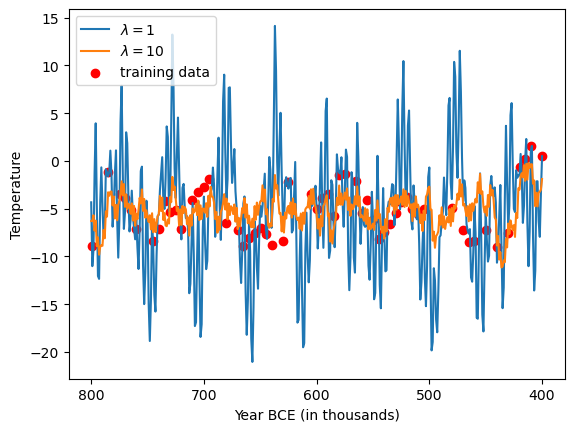
\includegraphics[width=.75\textwidth]{img_output/p4.5.png}
\end{center}

\noindent Errors, alongside the unregularized basis (d) model from Problem 3:
\begin{center}
\begin{tabular}{lcccc}
  \hline
  Model & Train MSE & Test MSE & $\|\boldw\|_2$ & Exact zeros \\
  \hline
  Vanilla basis (d)      & $0.6432$ & $58.9446$ & $3.85\times 10^{5}$ & $0/50$ \\
  LASSO, $\lambda = 1$   & $1.9509$ & $30.0606$ & $9.36$  & $10/50$ \\
  LASSO, $\lambda = 10$  & $3.1365$ & $\mathbf{15.6184}$ & $5.58$  & $19/50$ \\
  \hline
\end{tabular}
\end{center}

\textbf{The graphs.} The unregularized basis (d) fit in Problem 3 swings between
roughly $\pm 30$, wildly overshooting between training points. The $\lambda = 1$
fit is visibly calmer but still oscillates over roughly $[-21, 14]$. The
$\lambda = 10$ fit is tamer again, mostly staying within $[-12, 2]$ and tracking
the band of training data rather than lurching past it. Increasing $\lambda$
monotonically damps the high-frequency oscillation.

\textbf{The errors.} Training MSE gets steadily \emph{worse} as $\lambda$ grows
($0.64 \to 1.95 \to 3.14$), which is expected --- we are no longer minimizing
training error alone, but training error plus a penalty. Test MSE improves
dramatically over the same range ($58.94 \to 30.06 \to 15.62$, a $3.8\times$
reduction). This is the bias--variance tradeoff made explicit: we deliberately
accept a worse fit to the training data in exchange for much better
generalization.

\textbf{Why it works.} The mechanism is visible in the last two columns. The
unregularized fit achieves its near-interpolation through enormous weights
($\|\boldw\|_2 \approx 3.9\times10^5$) that cancel against one another --- exactly
at the training points, and nowhere else. The $\ell_1$ penalty makes that
cancellation expensive, collapsing $\|\boldw\|_2$ to single digits. LASSO
additionally drives coordinates to \emph{exactly} zero ($10$ of $50$ at
$\lambda=1$, $19$ of $50$ at $\lambda=10$), performing feature selection by
discarding whole cosine frequencies. Ridge would shrink these weights but leave
them nonzero; this sparsity is the distinctive consequence of the Laplace prior
from part 3.

\textbf{But regularization does not rescue a bad basis.} Even the better model
($15.62$) remains worse than simply predicting the test mean ($9.07$), and far
worse than basis (c) from Problem 3 ($5.97$) or kernelized regression from
Problem 1 ($1.86$). Regularization substantially repairs an over-parameterized
model, but choosing an appropriately sized basis in the first place beats
over-fitting and then penalizing. The monotone improvement from $\lambda = 1$ to
$\lambda = 10$ also suggests the optimum lies at larger $\lambda$ still, which
is a reminder that $\lambda$ is a hyperparameter to be selected on validation
data, not fixed arbitrarily.

\noindent\emph{Two implementation notes.} (i) The first coordinate is the bias
column and is updated without soft-thresholding, as the algorithm specifies;
penalizing the intercept would make the fit depend on the arbitrary origin of
the temperature scale. (ii) At $\lambda = 10$ coordinate descent converged after
$838$ sweeps, whereas at $\lambda = 1$ it was still moving when the $5000$-iteration
cap was reached --- stronger regularization pins more coordinates at zero and
converges faster.\footnote{The provided \texttt{preprocess\_lasso} standardizes
whichever array it is given using that array's own column statistics, so the
test inputs are standardized by test rather than training statistics. The
figures above use the helper as provided; standardizing the test set with the
training statistics instead gives $31.14$ and $16.11$, leaving every conclusion
unchanged.}

\end{enumerate}

\end{solution}

%%%%%%%%%%%%%%%%%%%%%%%%%%%%%%%%%%%%%%%%%%%%%
% Name and Calibration
%%%%%%%%%%%%%%%%%%%%%%%%%%%%%%%%%%%%%%%%%%%%%
\newpage

\textbf{Name}:

\textbf{Collaborators and Resources}:

\end{document}
